% ============================================================
%  研究专题稿（格式同《校级优秀毕业论文选编》电子版）
%  题目：基于可微物理的四足接触动力学神经残差——误差通道匹配与梯度保真
%  作者：徐路（自动化2202）  指导教师：李艳君、蔡永斌
%  编译：xelatex（2轮）；本地预览见 build_preview.sh（Noto 替身字体）
% ============================================================
\documentclass[zihao=5, a4paper]{ctexart}

% ---------- 页面：A4，上下左右 2.5cm ----------
\usepackage[a4paper, top=2.5cm, bottom=2.5cm, left=2.5cm, right=2.5cm, footskip=1.0cm]{geometry}
\linespread{1.0}\setlength{\parindent}{2em}

% ---------- 字体（权威：宋体/黑体/楷体；预览由脚本替换为 Noto）----------
\setmainfont{Times New Roman}
\setCJKmainfont{SimSun}[AutoFakeBold=2.5]
\setCJKfamilyfont{zhsong}{SimSun}[AutoFakeBold=2.5]
\setCJKfamilyfont{zhhei}{SimHei}
\setCJKfamilyfont{zhkai}{KaiTi}

% ---------- 数学/图表 ----------
\usepackage{amsmath, amssymb, bm}
\usepackage{graphicx}\graphicspath{{figures/}}
\usepackage{booktabs, array, caption}
\usepackage{placeins}
\captionsetup{labelsep=quad, font=small}

% ---------- 小标题：黑体五号顶格；一、二… / 1．2．----------
\ctexset{
  section   = {name={,、}, number=\chinese{section}, format=\heiti\zihao{5}\raggedright, beforeskip=8pt, afterskip=4pt, indent=0pt},
  subsection= {name={,．}, number=\arabic{subsection}, format=\heiti\zihao{5}\raggedright, beforeskip=6pt, afterskip=3pt, indent=0pt},
}

% ---------- 页码：小五号，底端居中 ----------
\usepackage{fancyhdr}
\pagestyle{fancy}\fancyhf{}\renewcommand{\headrulewidth}{0pt}
\fancyfoot[C]{\zihao{-5}\thepage}

\usepackage[hidelinks]{hyperref}
\usepackage[capitalise, noabbrev]{cleveref}
\crefname{figure}{图}{图}\Crefname{figure}{图}{图}
\crefname{table}{表}{表}\Crefname{table}{表}{表}

\newcommand{\gdiff}{g_{\mathrm{diff}}}

\begin{document}

% ===================== 题目区 =====================
\thispagestyle{fancy}
{\zihao{5}\ }

\begin{center}
  {\heiti\zihao{-2} 基于可微物理的四足接触动力学神经残差：\\误差通道匹配与梯度保真}
\end{center}

{\zihao{5}\ }

\begin{center}\kaishu\zihao{5}\bfseries
\begin{tabular}{@{}r@{\hspace{2.5em}}l@{}}
自动化2202班 & 徐\quad 路 \\[3pt]
指导教师 & 李艳君\quad 蔡永斌 \\
\end{tabular}
\end{center}

{\zihao{5}\ }

% ===================== 中文摘要 =====================
\noindent{\heiti\zihao{5} 摘\hspace{1em}要：}{\kaishu\zihao{5} 可微物理为无人机端到端训练提供了高样本效率的密集一阶梯度，但迁移到四足机器人时，足端接触同时破坏"光滑性"与"可微平坦性"，使反向传播（BPTT）梯度幅值爆炸、方向失真。一条折中路线是"物理模型$+$神经残差"$a=a_{\text{phys}}+r_\phi$，以数据补偿物理模型失配。本文在最小可微平面单刚体模型（SRBM）上系统研究该路线，核心关切不是残差的\textbf{前向拟合精度}，而是其\textbf{梯度保真}——可微训练用的正是经 BPTT 的梯度，残差若"前向准而梯度错"，反会训出更差的策略。借助"用参数失配构造可微 teacher、其真梯度可解析获得"这一方法学设计，本文定量比较了加速度残差、接触力残差、约束接触力残差、运动学（落足）残差及力$+$运动学双头组合残差，在\textbf{参数、小几何、极端几何与未知混合}四类失配下的前向精度、梯度保真与闭环可迁移性。主要发现：（1）前向精度$\neq$梯度保真，存在"前向更低、梯度更差"的反例；（2）残差必须参数化在\textbf{误差真正发生的物理位置}——力律误差用接触力残差、几何误差用运动学残差，放错位置则梯度必崩、并在闭环策略质量上被放大；（3）当几何失配大到\textbf{翻转接触力臂符号}，编码标称几何的接触力残差从最优沦为最差，须改用运动学残差；（4）事先不知失配类型时，双头残差能\textbf{自动把修正路由到正确通道}，在三类失配上梯度保真均$\ge$0.995、闭环部署均达 oracle 水平。本文为可微物理在接触系统上的迁移给出了"残差选型"的清晰原理与可复现的最小实验。}

{\kaishu\zihao{5}\noindent{\heiti 关键词：}可微物理；四足机器人；神经残差；梯度保真；接触动力学}

\vspace{2pt}

% ===================== 英文摘要 =====================
\noindent{\bfseries\zihao{5} Abstract:~}{\zihao{5} Differentiable physics offers dense, sample-efficient first-order gradients for end-to-end UAV training, but porting it to legged robots is hard: foot contact breaks both smoothness and differential flatness, making back-propagated (BPTT) gradients blow up in magnitude and err in direction. A pragmatic route is the ``physics$+$neural residual'' model $a=a_{\text{phys}}+r_\phi$, which uses data to compensate model mismatch. On a minimal differentiable planar single-rigid-body model (SRBM), this paper studies that route with a central concern that is \emph{gradient fidelity} rather than \emph{forward accuracy}: differentiable training consumes BPTT gradients, so a residual that is ``forward-accurate yet gradient-wrong'' trains a worse policy. Exploiting a methodological trick---building a differentiable teacher by parameter mismatch so its true Jacobian is analytic---we compare acceleration, contact-force, constrained contact-force, kinematic (foot-placement), and force$+$kinematic dual-head residuals across four mismatch types (parametric, mild-geometric, extreme-geometric, unknown-mixed). Key findings: (1) forward accuracy $\neq$ gradient fidelity, with explicit ``lower-forward-yet-worse-gradient'' counterexamples; (2) a residual must be parameterized \emph{where the error actually lives}---force errors via a contact-force residual, geometric errors via a kinematic residual---else the gradient breaks and the failure is amplified in closed-loop policy quality; (3) when geometric mismatch is large enough to \emph{flip the contact moment-arm sign}, the contact-force residual that hard-codes nominal geometry turns from best to worst, and a kinematic residual is required; (4) when the mismatch type is unknown, a dual-head residual \emph{auto-routes} the correction to the correct channel, attaining gradient cosine $\ge$0.995 and oracle-level closed-loop deployment on all three mismatch types.}

{\zihao{5}\noindent{\bfseries Key words:~}Differentiable Physics; Legged Robots; Neural Residual; Gradient Fidelity; Contact Dynamics}

\vspace{4pt}

% ===================== 一、绪论 =====================
\section{绪论}

将感知到控制的映射端到端地学习出来，是自主机器人的核心范式之一。深度强化学习（RL）以标量奖励的零阶估计优化任务级目标，泛化能力强，但通常需数万次交互才能收敛\cite{ref8,ref11}。\textbf{可微物理}（differentiable simulation）将仿真过程构建为完全可微的计算图，损失梯度可经动力学直接反向传播，提供密集且方向确定的一阶梯度并隐含动力学先验，样本效率显著更高\cite{ref13}。其代表性工作 DiffPhysDrone\cite{ref14} 在无人机视觉避障上以约 10\% 的 PPO 样本量达到约 90\% 成功率，关键之一是其点质量动力学的\textbf{可微平坦性}：姿态可由推力向量\textbf{代数反解}，使从控制到状态的整条计算图光滑可导。

然而，将这一路线迁移到\textbf{四足机器人}并不平凡，核心障碍是\textbf{接触}。与无人机不同，四足的姿态不再能代数反解，而是由\textbf{接触力矩二阶产生}（$I\ddot\theta=\sum_i \bm r_i\times\bm F_i$）；且足端接触切换与摩擦锥引入新的\textbf{非光滑}。其后果是可微平坦性丧失、BPTT 梯度沿展开步数的谱半径超过 1 时方差指数增长\cite{ref12}：在刚性接触下梯度幅值可爆炸数千倍、方向出现大比例错误，这正是可微物理编程中普遍观察到的训练不稳定\cite{ref29}。应对接触梯度病理有两条思路：其一是\textbf{光滑化接触}（解析平滑罚函数、维持预定接触序列），如 Song 等\cite{ref13} 在可微仿真中训练四足运动；其二是\textbf{用神经网络补偿物理模型的失配}，即"物理模型$+$神经残差"$a=a_{\text{phys}}+r_\phi(x,u)$，在保留物理先验"方向正确的骨架"的同时，用数据校正幅值与细节。本文聚焦后者。

残差路线的真正风险并不在前向拟合，而在\textbf{梯度}。可微训练消费的是经 BPTT 的梯度；一个把动力学\emph{值}拟合得很准、但其\emph{导数}（雅可比）方向错误的残差，会给出"自信却错误"的梯度，反而把策略训练带偏——Metz 等\cite{ref12} 已从理论上指出可微估计的梯度偏差问题。因此本文的核心关切被明确为\textbf{梯度保真}（gradient fidelity），而非前向精度。为使"梯度保真"可被\textbf{直接量化}，本文采用一个方法学设计：用\textbf{参数失配}的可微 SRBM 充当 teacher——由于 teacher 本身可微，其"真梯度"$J_T=\partial a_T/\partial(x,u)$ 解析可得，于是任一残差 student 的雅可比可与之逐元比较，无需引入不可微的高保真仿真器。

本文贡献如下：（1）在最小 SRBM 上\textbf{定量刻画"前向精度$\neq$梯度保真"}，给出"前向更低、梯度更差"的反例；（2）提出并验证\textbf{残差选型原理}——残差必须参数化在误差真正发生的物理位置（力律误差$\to$接触力残差、几何误差$\to$运动学残差），并以接触门控、平滑摩擦锥、乘性限幅等\textbf{可微物理约束}近乎零（梯度）成本地保证物理合法性；（3）以\textbf{力臂符号翻转}为临界，\textbf{界定}"残差越物理越可信"的适用边界——失配大到翻转力臂时，编码标称几何的力残差反而最差；（4）给出\textbf{双头自动路由}的收尾方案，在未知失配类型下统一三类失配，并以闭环部署与正则化鲁棒性加以确证。本文方法与实验完全在可复现的开源 SRBM 平台上完成。

% ===================== 二、可微SRBM动力学与接触梯度病理 =====================
\section{可微 SRBM 动力学与接触梯度病理}

\subsection{平面单刚体模型与可微接触}

为在保持可微、可解析的前提下抓住四足区别于无人机点质量的本质，本文采用\textbf{平面单刚体模型}（SRBM，Song 等\cite{ref13} 浮动基 SRBD 的二维退化）。状态 $\bm x=[p_x,p_z,\theta,v_x,v_z,\omega]$（机身质心位置、俯仰角、线/角速度），控制为两条棱柱腿的伸长量 $\mathrm{ext}_k$；差动伸长产生俯仰力矩。足端经旋转 $R(\theta)$ 投影到世界系，穿地时产生\textbf{平滑罚函数法向力}与\textbf{平滑库仑摩擦}：
\begin{equation}
  F_n=\mathrm{clamp}\!\big(k_n\,\varepsilon\,\mathrm{softplus}(-f_z/\varepsilon)-k_d\,\dot d\,\sigma(-f_z/\varepsilon),\,0\big),
  \qquad
  F_t=-\mu F_n\tanh(v_t/v_\varepsilon),
  \label{eq:contact}
\end{equation}
其中 $f_z$ 为足端高度、$\sigma$ 为接触门控。整段动力学以显式积分推进、对控制与参数可导。该模型\textbf{最小地}保留了四足的两个本质特征：其一，\textbf{姿态由接触力矩二阶产生}
\begin{equation}
  I\ddot\theta=\tau=\sum_{i} \big(r_{x,i}F_{n,i}-r_{z,i}F_{t,i}\big),\qquad \bm r_i=\bm p_{\text{foot},i}-\bm p_{\text{com}},
  \label{eq:torque}
\end{equation}
不能像无人机那样代数反解，可微平坦性丧失；其二，\textbf{前向推进只能靠切向摩擦}，接触切换与摩擦锥引入新的非光滑。

\subsection{接触梯度病理与本文的诊断量}

\cref{fig:srbm} 给出 SRBM 姿态动力学的两个签名：俯仰相图 $\theta$--$\omega$ 是二阶 ODE 的收敛螺旋（对照无人机的代数解姿态），且\textbf{终端姿态对腿伸长的灵敏度铺满整段历史}（敏感度质心远离终点）——这正是可微平坦性丧失的定量表现。进一步，在\textbf{刚性}接触下，整段 BPTT 的梯度范数较平滑接触爆炸约三个数量级、且出现大比例方向错误；而无人机式的时间梯度衰减（GDecay）与全局梯度范数裁剪本质是\textbf{正标量缩放}，只能"压幅"不能"纠偏"（符号不一致率严格不变）。这两点共同决定：残差路线宜建立在\textbf{平滑}接触之上（梯度有界），而模型与真实之间的\textbf{失配}则交给神经残差补偿——于是问题归结为"补偿得对不对"，即\textbf{梯度保真}。

\begin{figure}[htbp]
  \centering
  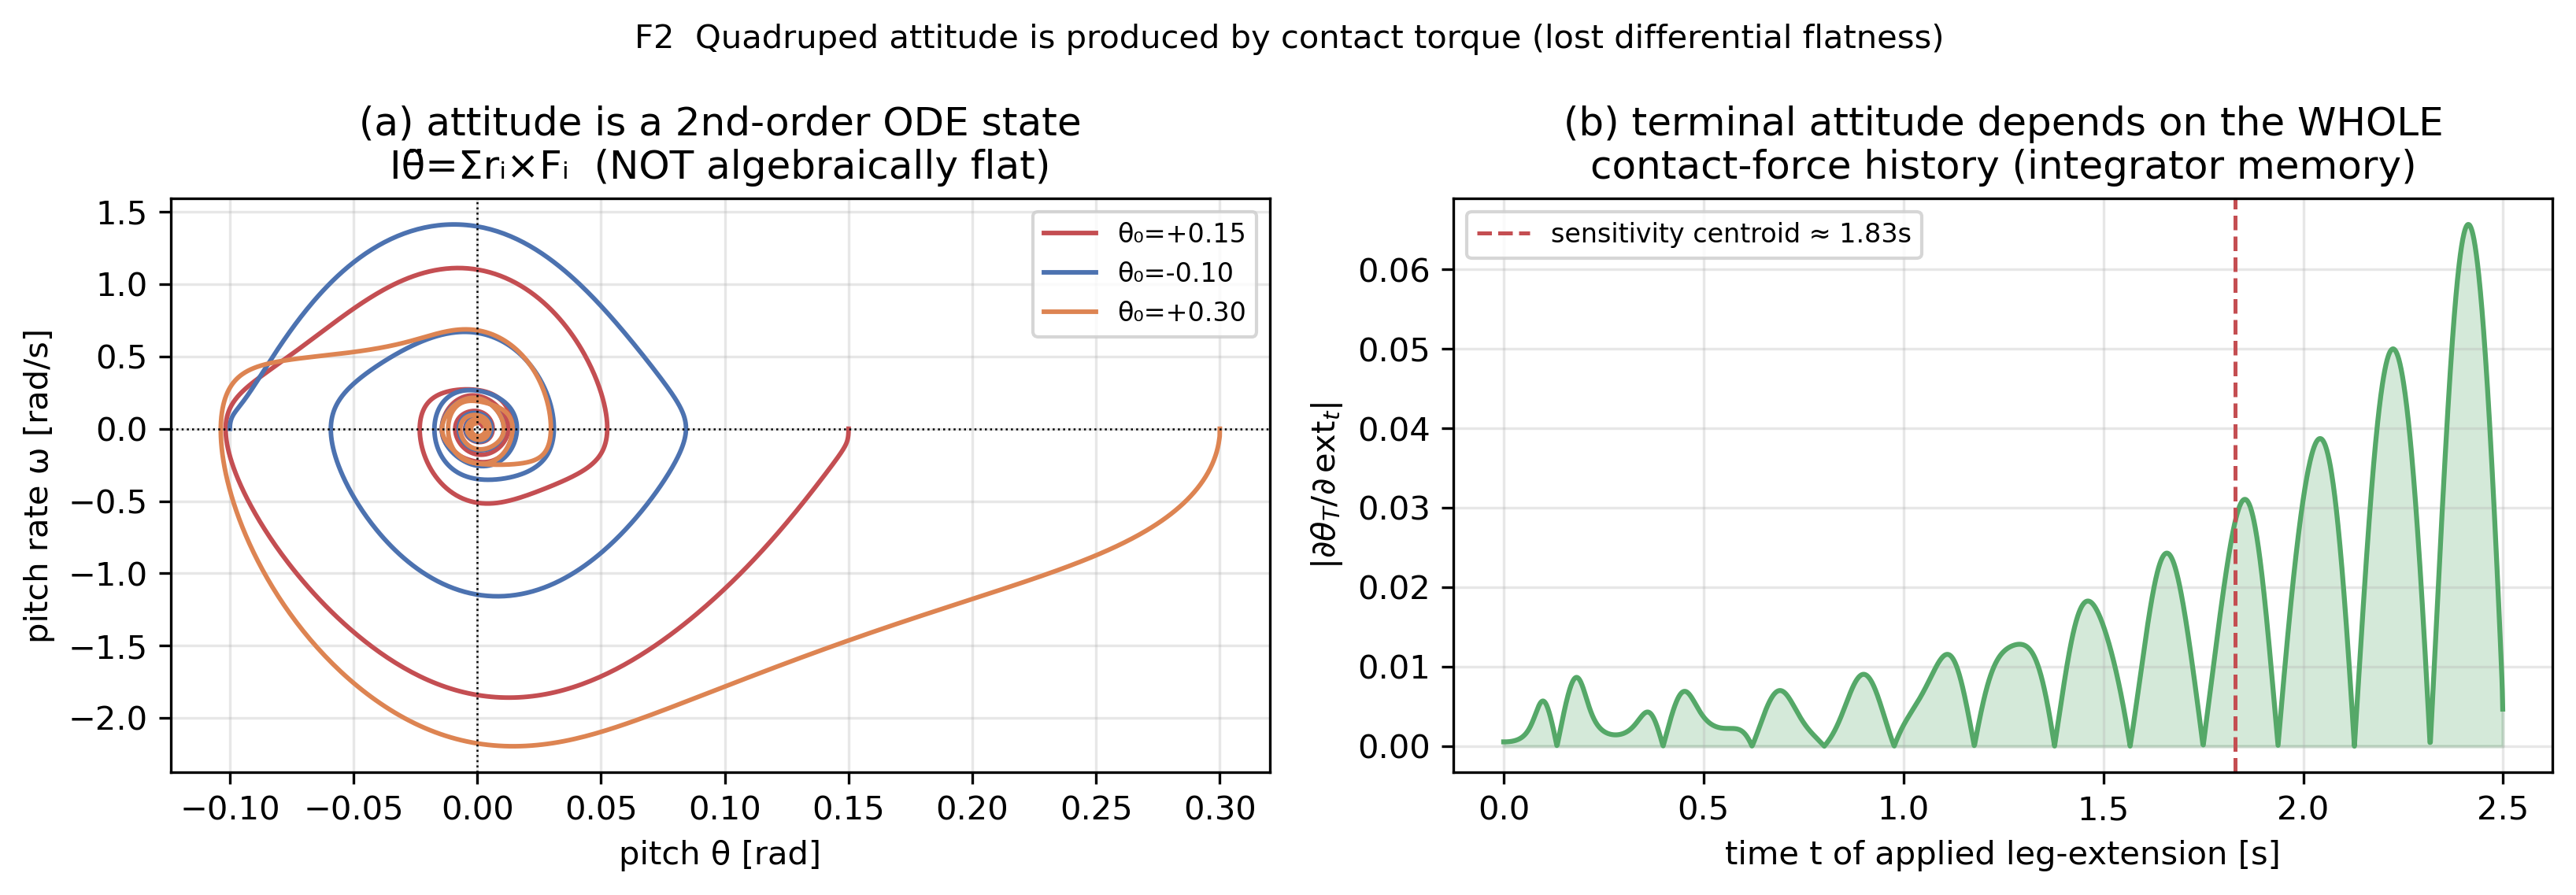
\includegraphics[width=0.96\textwidth]{F2_attitude.png}
  \caption{SRBM 姿态动力学的接触梯度签名。左：俯仰相图为二阶 ODE 收敛螺旋（$I\ddot\theta=\sum r\times F$），区别于无人机的代数解姿态；右：终端姿态对腿伸长的灵敏度铺满整段历史，是可微平坦性丧失的定量签名，也是接触使梯度变"长程耦合"的来源。}
  \label{fig:srbm}
\end{figure}

\subsection{可微 teacher 与梯度保真的量化协议}

本文用\textbf{参数失配}的可微 SRBM 作 teacher：student 用标称参数 $(m,I,k_n,k_d,\mu)$ 加残差，teacher 用真实（失配）参数。由于 teacher 可微，其真梯度 $J_T=\partial a_T/\partial(\bm x,\bm u)\in\mathbb R^{3\times8}$ 解析可得。评估协议据此定义四个层次的诊断量：\textbf{前向 RMS}（$\|a_S-a_T\|$）、\textbf{梯度余弦}（$\langle J_S,J_T\rangle$，及限定到姿态行$\times$控制列的\textbf{姿态梯度余弦}）、\textbf{差动控制增益} $\gdiff\equiv\partial\alpha/\partial\mathrm{ext}_0-\partial\alpha/\partial\mathrm{ext}_1$（其符号即平衡控制方向）、以及\textbf{经 rollout 的 BPTT 梯度}与\textbf{闭环部署 loss}。其中前向与梯度的\emph{背离}是全文的主线证据。

% ===================== 三、神经残差形式与物理约束 =====================
\section{神经残差形式与可微物理约束}

本文比较五种残差形式，其差别全在\textbf{把修正参数化在何处}（\cref{tab:forms}）。

\begin{table}[htbp]
  \centering
  \caption{五种神经残差形式（差别在修正注入的物理位置）}
  \label{tab:forms}
  \small\setlength{\tabcolsep}{6pt}
  \begin{tabular}{lll}
    \toprule
    残差形式 & 修正对象 & 物理约束 \\
    \midrule
    加速度残差 & 直接加到 $a$ & 无（最自由） \\
    接触力残差 & 每足 $\Delta F_n,\Delta F_t$ & 接触门控 + 法向非负 \\
    约束接触力残差 & 同上 & 乘性有界法向 + 平滑摩擦锥 + 限幅 \\
    运动学（落足）残差 & 每足接触点 $\Delta x$ & 经修正力臂 $r_x{+}\Delta x$ 算力矩 \\
    力 $+$ 运动学双头 & $\Delta F$ 与 $\Delta x$ 并存 & 上述之并，数据自动路由 \\
    \bottomrule
  \end{tabular}
\end{table}

\textbf{接触力残差}把修正放在每足接触力上（最贴近 SRBM 不准的源头 $k_n,k_d,\mu$），并以两条\textbf{结构性约束}保证物理合法：\textbf{接触门控} $\Delta F^\ast=\sigma(-f_z/\varepsilon)\Delta F$ 使离地时残差力$\to$0（不凭空给地面力），\textbf{法向非负}保证不被地面"吸住"。\textbf{约束接触力残差}进一步以\textbf{乘性有界}法向与\textbf{平滑摩擦锥}从结构上封死"残差接管"与"无正压力的摩擦"：
\begin{equation}
  F_n=F_n^{\text{phys}}\big(1+\alpha\tanh(\Delta F_n)\big)\ (\alpha{=}0.6),
  \qquad
  F_t=\mu F_n\tanh\!\Big(\tfrac{F_t^{\text{phys}}+\text{gate}\cdot\Delta F_t}{\mu F_n+\varepsilon}\Big),
  \label{eq:constrained}
\end{equation}
前者令法向最多被修正 $\pm60\%$（非负、限幅、$F_n^{\text{phys}}{=}0$ 时自动归零），后者令 $|F_t|\le\mu F_n$ 结构成立。\textbf{运动学残差}则把修正放在\textbf{接触点位置}：小网络输出每足落足偏置 $\Delta x_k$，在\textbf{修正后的落足点}跑同一套平滑接触模型，使力矩经\textbf{修正后的力臂} $r_x{+}\Delta x$ 流动。\textbf{双头组合残差}同时具备力头与运动学头，由前向回归\textbf{自动分配}修正，并可加 $L_2$ 正则 $\lambda_{\text{kin}}\|\Delta x\|^2+\lambda_{\text{force}}\|\Delta F\|^2$ 抑制过参数化。所有残差末层\textbf{零初始化}（起点即标称物理），训练用逐维归一化 MSE 以免被刚性法向加速度主导。

% ===================== 四、实验 =====================
\section{实验结果与分析}

\subsection{实验设置}

实验在 RTX 3080/3060 上以 \texttt{float64}、\texttt{cuda:0} 完成。标称 SRBM 参数 $m{=}10,I{=}0.35,k_n{=}6000,k_d{=}30,\mu{=}0.9,\text{half\_len}{=}0.25$；teacher 据实验取参数失配（如 $m{=}16,k_n{=}1.4\times10^4,\mu{=}0.45$）或几何失配（足端偏置 $\delta x$）。除特别说明外，残差以前向回归训练，再以上述协议在固定评估集上比较。训练种子固定（$\text{seed}{=}0$），确定性的梯度类结论跨运行稳定。

\subsection{前向精度 $\neq$ 梯度保真（R1--R2）}

第一组实验隔离最干净的\textbf{加速度残差}，对比两种 teacher 数据源。结果（\cref{tab:r1}，\cref{fig:r1}）给出全文的奠基性观察：对\textbf{平滑}（参数失配）teacher，残差既降前向误差又\textbf{改善}梯度（余弦 $0.954\!\to\!0.976$），是良性的；对\textbf{硬接触} teacher，残差前向几乎拟合不动，却把梯度余弦\textbf{腐蚀}到 $0.666$。尤为关键的是：硬 teacher 残差\textbf{前向误差更低}（13.8<15.5）却\textbf{梯度更差}——这构成"\textbf{前向准 $\neq$ 梯度准}"的直接反例，证明\textbf{不能用前向误差判断残差好坏}。经 rollout 的 BPTT 梯度（R2）进一步显示：平滑 teacher 残差的梯度即便经过多步展开仍紧贴真值，硬 teacher 残差则偏离——这是最贴近可微训练实际用途的检验。

\begin{table}[htbp]
  \centering
  \caption{加速度残差：前向精度、梯度保真与接管比（R1）}
  \label{tab:r1}
  \small\setlength{\tabcolsep}{10pt}
  \begin{tabular}{lccc}
    \toprule
    配置 & 前向 RMS & 梯度余弦（vs 真 $J_T$）& 接管比 $\|r_\phi\|/\|a_N\|$ \\
    \midrule
    未校正 nominal & 15.5 & 0.954 & --- \\
    残差（平滑 teacher）& \textbf{6.3} & \textbf{0.954$\to$0.976} & 0.14 \\
    残差（硬接触 teacher）& 13.8 & 0.954$\to$\textbf{0.666} & 0.26 \\
    \bottomrule
  \end{tabular}
\end{table}

\begin{figure}[htbp]
  \centering
  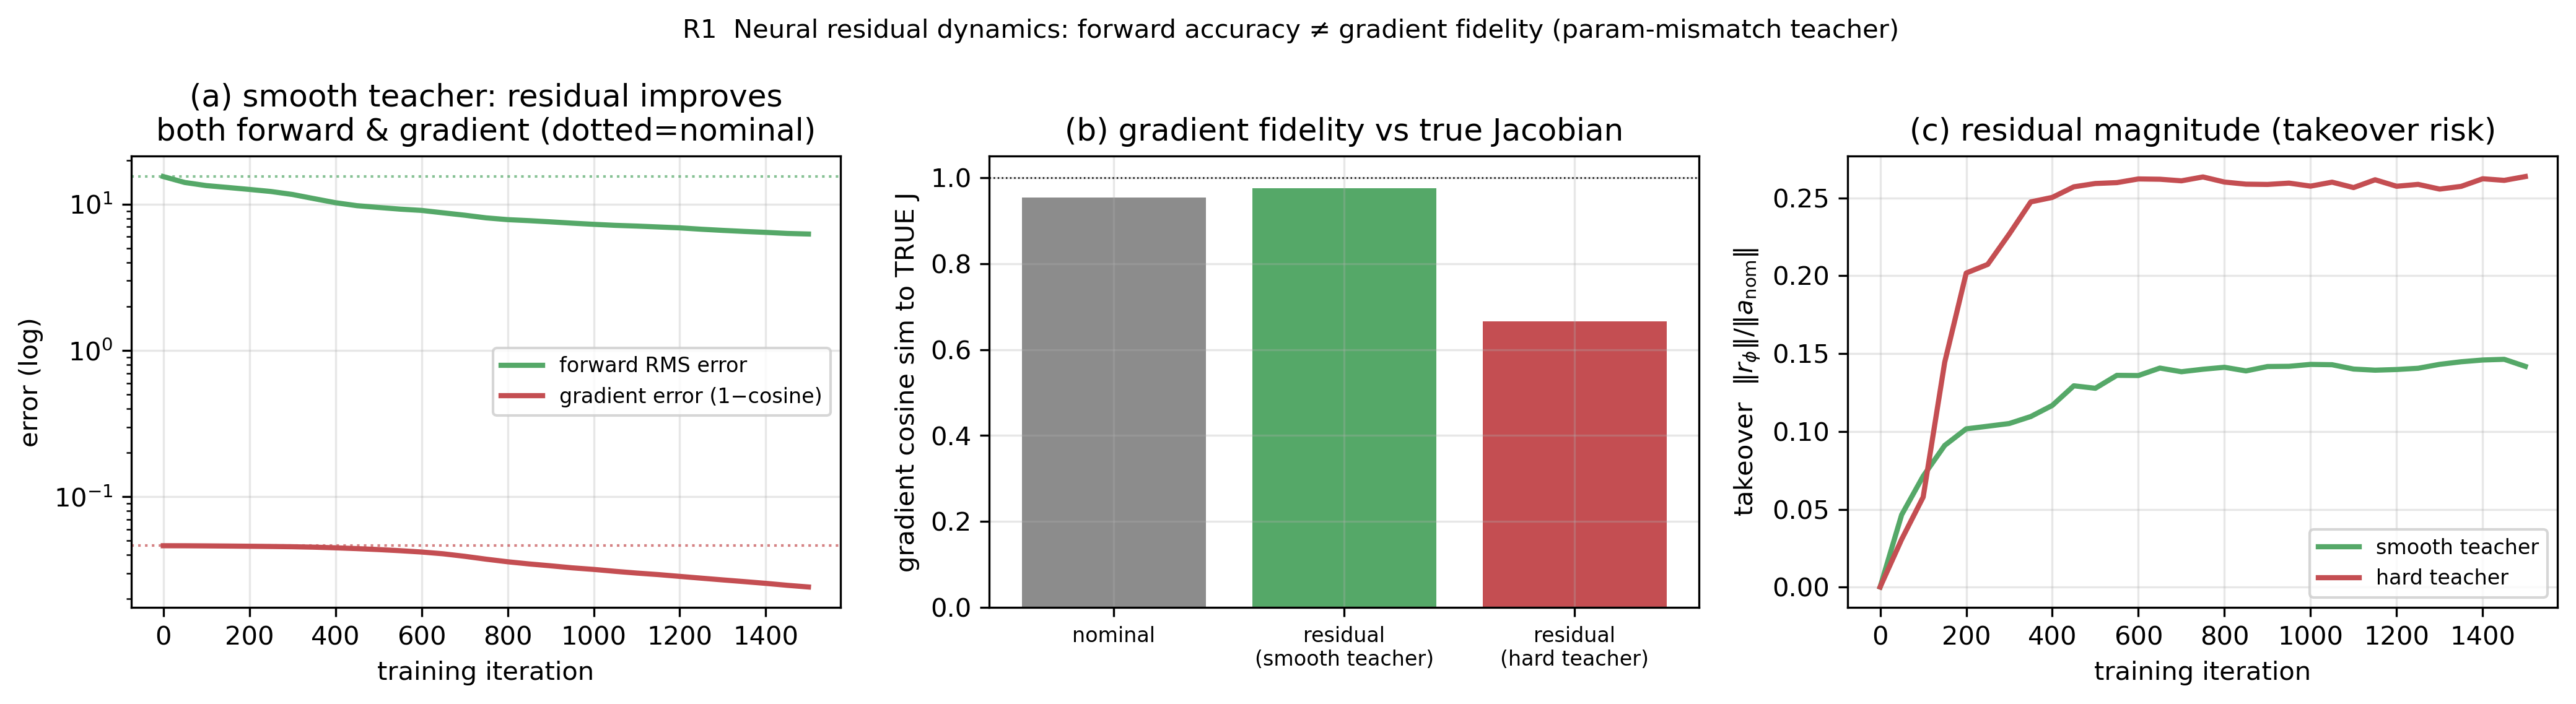
\includegraphics[width=0.95\textwidth]{R1_residual_gradfidelity.png}
  \caption{加速度残差的前向精度与梯度保真。平滑（参数失配）teacher 下残差改善梯度；硬接触 teacher 下残差前向尚可却腐蚀梯度——"代理可微 $\neq$ 真实可微"被定量复现。}
  \label{fig:r1}
\end{figure}

\subsection{残差形式与物理约束（R3--R4）}

把残差从加速度移到\textbf{接触力}（误差真正发生处），前向与梯度\textbf{双双更优}：接触力残差前向 3.2、梯度余弦 \textbf{0.998}，均优于加速度残差（6.3 / 0.969）（\cref{tab:r3}，\cref{fig:r3}）。\textbf{接触门控}的价值是\textbf{结构性}的：在留出的"明确离地"状态集上，门控版法向力 $\approx$0，无门控版\textbf{凭空给出 1.4\,N} 地面力，而门控\textbf{几乎不损梯度保真}（0.998 vs 0.996）——离地零力是结构保证，不依赖训练数据覆盖。约束接触力残差（R4）再加平滑摩擦锥与乘性限幅：无约束残差在约 86\% 样本上违反摩擦锥（离地处"无正压力的摩擦"）、并\textbf{接管}主模型（相对修正 4--9 倍），R4 则结构性地把锥违反压到 \textbf{0}、接管封顶 $\pm60\%$，且\textbf{几乎不损梯度保真}（余弦 0.999$\to$0.989）。需诚实指出：结构约束\textbf{本质是编码先验}，先验过紧（如锥 $\mu$ 小于真实摩擦）会削掉合法力、抬高前向误差，故约束的 $\mu$/限幅应取宽松或可学习。

\begin{table}[htbp]
  \centering
  \caption{残差参数化位置对前向与梯度的影响（R3）}
  \label{tab:r3}
  \small\setlength{\tabcolsep}{9pt}
  \begin{tabular}{lccc}
    \toprule
    残差形式 & 前向 RMS & 梯度余弦 & 离地幻影法向力 \\
    \midrule
    未校正 nominal & 15.9 & 0.941 & --- \\
    加速度残差 & 6.3 & 0.969 & --- \\
    接触力残差·门控 & \textbf{3.2} & \textbf{0.998} & \textbf{0.017\,N} \\
    接触力残差·无门控 & --- & 0.996 & 1.41\,N \\
    \bottomrule
  \end{tabular}
\end{table}

\begin{figure}[htbp]
  \centering
  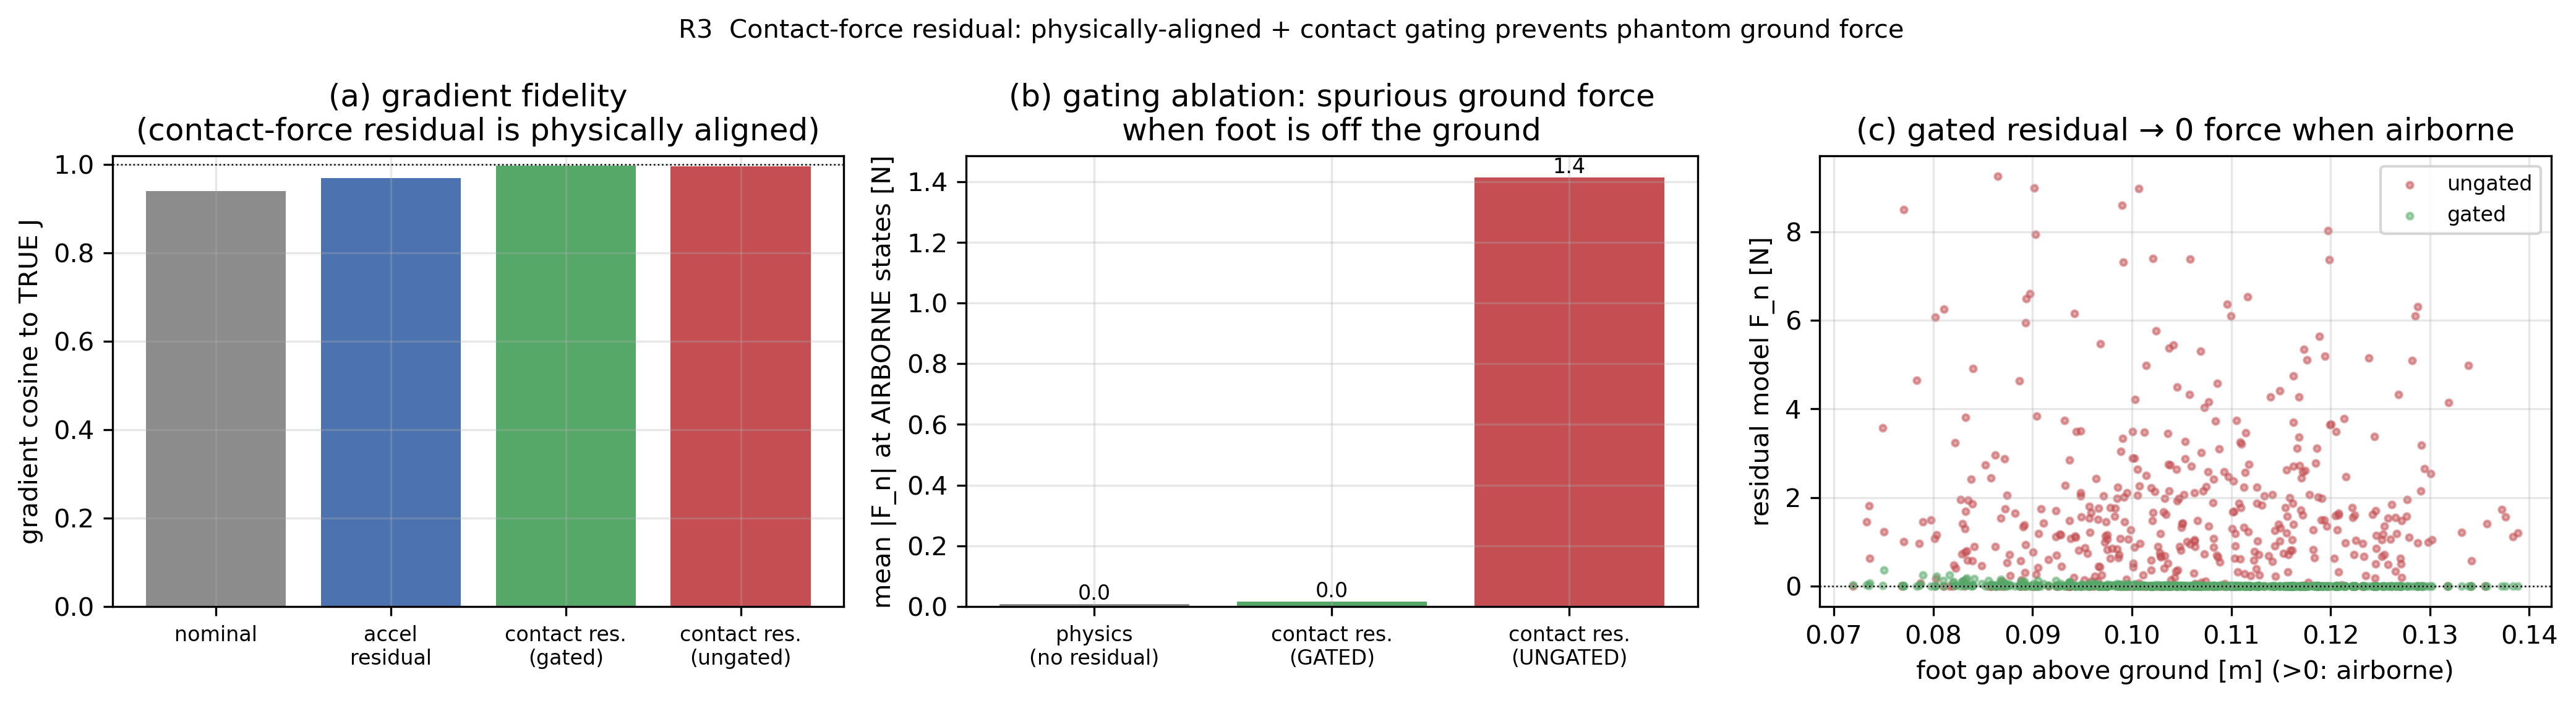
\includegraphics[width=0.95\textwidth]{R3_contact_residual.png}
  \caption{接触力残差（门控 + 法向非负）。把残差放在误差发生处使前向与梯度双双更优；门控在留出的离地集上结构性地消除幻影地面力，几乎不损梯度保真。}
  \label{fig:r3}
\end{figure}

\subsection{几何失配与"物理结构"的边界（R5、R8）}

\textbf{结构性几何失配}（足端偏置）比缩放型参数失配更狠，因其改变力矩臂 $r_x$、最易破坏\textbf{姿态}梯度方向。在\textbf{小}失配（对称 $\delta x{=}0.06$）下，自由加速度残差前向拟合最好却把姿态梯度余弦腐蚀到 $0.927$（\textbf{比 nominal 的 0.968 还差}），而物理结构化的接触力残差保住姿态梯度（0.978）——又一"前向 $\neq$ 梯度"反例，且专打姿态。然而这一保护\textbf{有边界}。本文用\textbf{非对称剪刀偏置} $\bm{fd}{=}[-\delta x,+\delta x]$ 使差动控制力臂 $r_{x0}-r_{x1}=2(\text{half\_len}-\delta x)$ 在 $\delta x{=}\text{half\_len}(0.25)$ 处\textbf{过零反号}（对称平移则该力臂差恒定、不翻转）。\cref{fig:r8} 显示：teacher 的差动控制增益 $\gdiff$ 随 $\delta x$ 单调下降、在 $\delta x{\approx}0.25$ 处\textbf{穿零变负}（控制方向整体翻转）；而约束接触力残差\textbf{只能缩放力、搬不动接触点}（其力矩恒用标称力臂 $r_x$），故\textbf{对符号翻转结构失明}——$\gdiff$ 死守正号、姿态梯度余弦塌到 0.31，\textbf{从最优沦为最差}；自由加速度残差因能拟合前向反而部分跟上翻转。这界定了"残差越物理越可信"的前提：\textbf{残差所编码的物理结构本身须近似正确}；一旦几何失配翻转力臂，焊死的标称力臂从"归纳偏置"变为"错误先验"。

\begin{figure}[htbp]
  \centering
  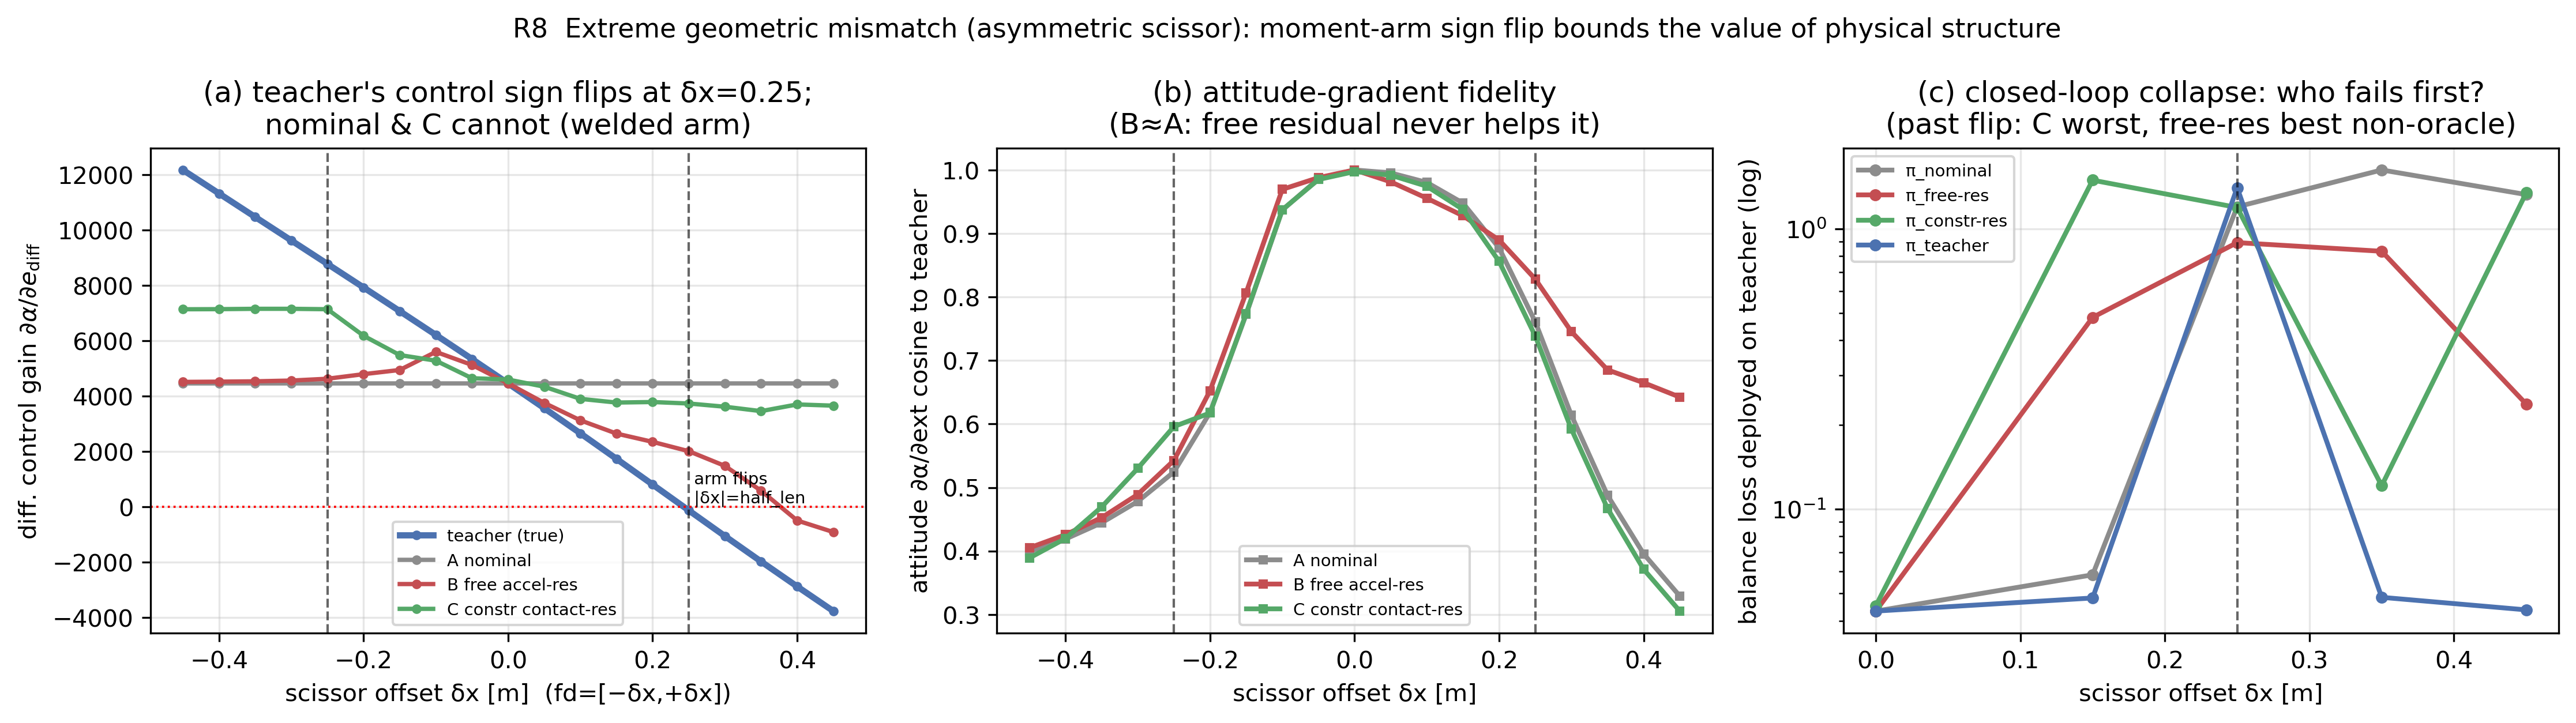
\includegraphics[width=0.97\textwidth]{R8_extreme_geometry.png}
  \caption{极端几何失配（非对称剪刀足偏，力臂符号翻转）。左：teacher 的差动控制增益在 $\delta x{=}0.25$ 处穿零反号，nominal 与约束接触力残差因焊死标称力臂而无法跟随。中：姿态梯度余弦——约束接触力残差在大失配区从最优掉到最差。右：闭环平衡 loss 在 $\delta x{=}0.25$ 处因支撑基退化而对任意策略奇异（含 oracle），故此处反映可控性而非残差质量。}
  \label{fig:r8}
\end{figure}

\subsection{运动学残差：把修正放回误差发生处（R9）}

R8 的诊断指向药方：力臂符号翻转是\textbf{运动学}失配，须\textbf{修正接触点位置}而非力。\textbf{运动学残差}让网络输出每足落足偏置 $\Delta x_k$，在修正后的落足点跑同一接触模型。结果\textbf{近乎完美}（\cref{fig:r9}）：其 $\gdiff$ 逐点贴合 teacher（$\delta x{=}0.45$：$-3680$ vs $-3696$，\textbf{随 teacher 一同穿零变负}），姿态梯度余弦在\textbf{全 $\delta x$ 区间恒为 1.00}（约束接触力残差在 $\delta x{=}0.45$ 仅 0.28），前向 RMS 也小 1--2 个数量级；闭环上，其策略在整个翻转后区间（$\delta x{=}0.35/0.40/0.45$）部署到真实 teacher 都稳定在 \textbf{oracle 水平}（$0.044$--$0.049$），是唯一能迁移过符号翻转的非 oracle。其近乎完美\textbf{部分得益于本实验的几何失配恰是运动学残差假设类内的常值落足偏置}；真实场景中落足误差可能随状态/地形变化，残差只能近似恢复——R9 证明的是"\textbf{参数化对上误差类型即可恢复梯度}"，而非"运动学残差对任意几何失配都完美"。

\begin{figure}[htbp]
  \centering
  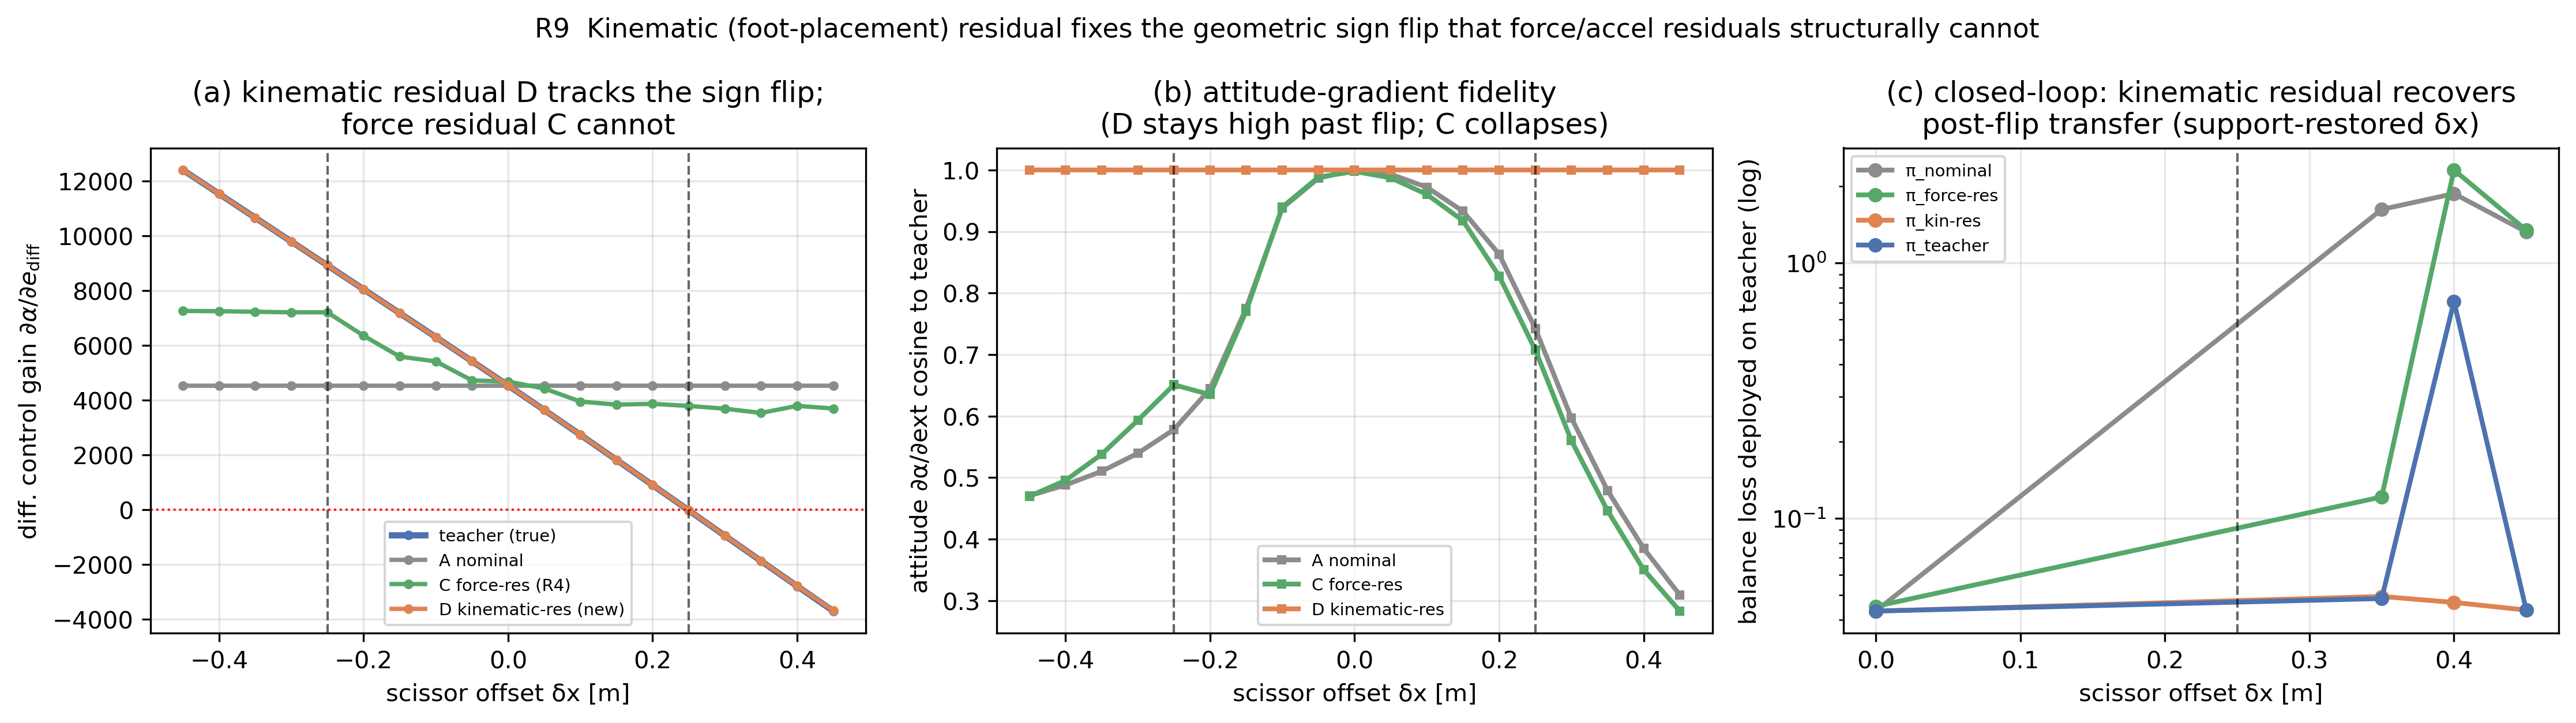
\includegraphics[width=0.97\textwidth]{R9_kinematic_residual.png}
  \caption{运动学（落足）残差治好几何符号翻转。左/中：其差动控制增益与姿态梯度余弦逐点贴合 teacher（余弦全程 1.00），而只能缩放力的接触力残差结构失明。右：闭环部署到翻转后的 teacher 全程达 oracle 水平。}
  \label{fig:r9}
\end{figure}

\subsection{未知失配下的双头自动路由与闭环 capstone（R10--R11）}

真实迁移中\textbf{事先不知}失配是力律还是几何。本文给残差\textbf{两个头}——力头（约束接触力残差）与运动学头（落足偏置），由前向回归自动分配。在\textbf{参数 / 几何 / 两者}三种 teacher 上（\cref{tab:r10}，\cref{fig:r10}）：每个\textbf{单头}都各栽一种失配（力头治力不治几何，且在力$+$几何同时失配时姿态梯度\textbf{变号} $-0.10$；运动学头治几何不治力），而\textbf{双头三种 teacher 上全梯度余弦均 $\ge$0.995}，并\textbf{自动路由}——几何 teacher 下运动学头学到 $|\Delta x|{=}0.350$（恰为真实 $\delta x{=}0.35$）、力头$\approx$0；参数 teacher 反之；两者并用。闭环上（R11，\cref{fig:r11}），双头策略部署到三种 teacher \textbf{全部 $\approx$ oracle}，使 R10 从"梯度 capstone"升级为"\textbf{闭环 capstone}"；加 $L_2$ 正则后路由\textbf{仍稳且更锐}（不需要的头压得更接近 0、梯度余弦仍 $\ge$0.99），证明自动路由\textbf{非无约束拟合的偶然}。需诚实指出：闭环平衡任务对\textbf{参数}误差反馈鲁棒，故其判别轴是几何、且单种子噪声较大，精细数值不宜逐位复现，确定性结论以梯度/路由量为准。

\begin{table}[htbp]
  \centering
  \caption{双头组合残差在三类 teacher 上的全梯度余弦（R10）}
  \label{tab:r10}
  \small\setlength{\tabcolsep}{12pt}
  \begin{tabular}{lccc}
    \toprule
    残差 & T\_force（参数）& T\_geom（几何）& T\_both（两者）\\
    \midrule
    C 力头 & 0.971 & 0.724 & 0.267（姿态 $-0.10$）\\
    D 运动学头 & 0.792 & \textbf{1.000} & 0.968 \\
    \textbf{E 双头（自动路由）}& \textbf{0.996} & \textbf{1.000} & \textbf{0.995} \\
    \bottomrule
  \end{tabular}
\end{table}

\begin{figure}[htbp]
  \centering
  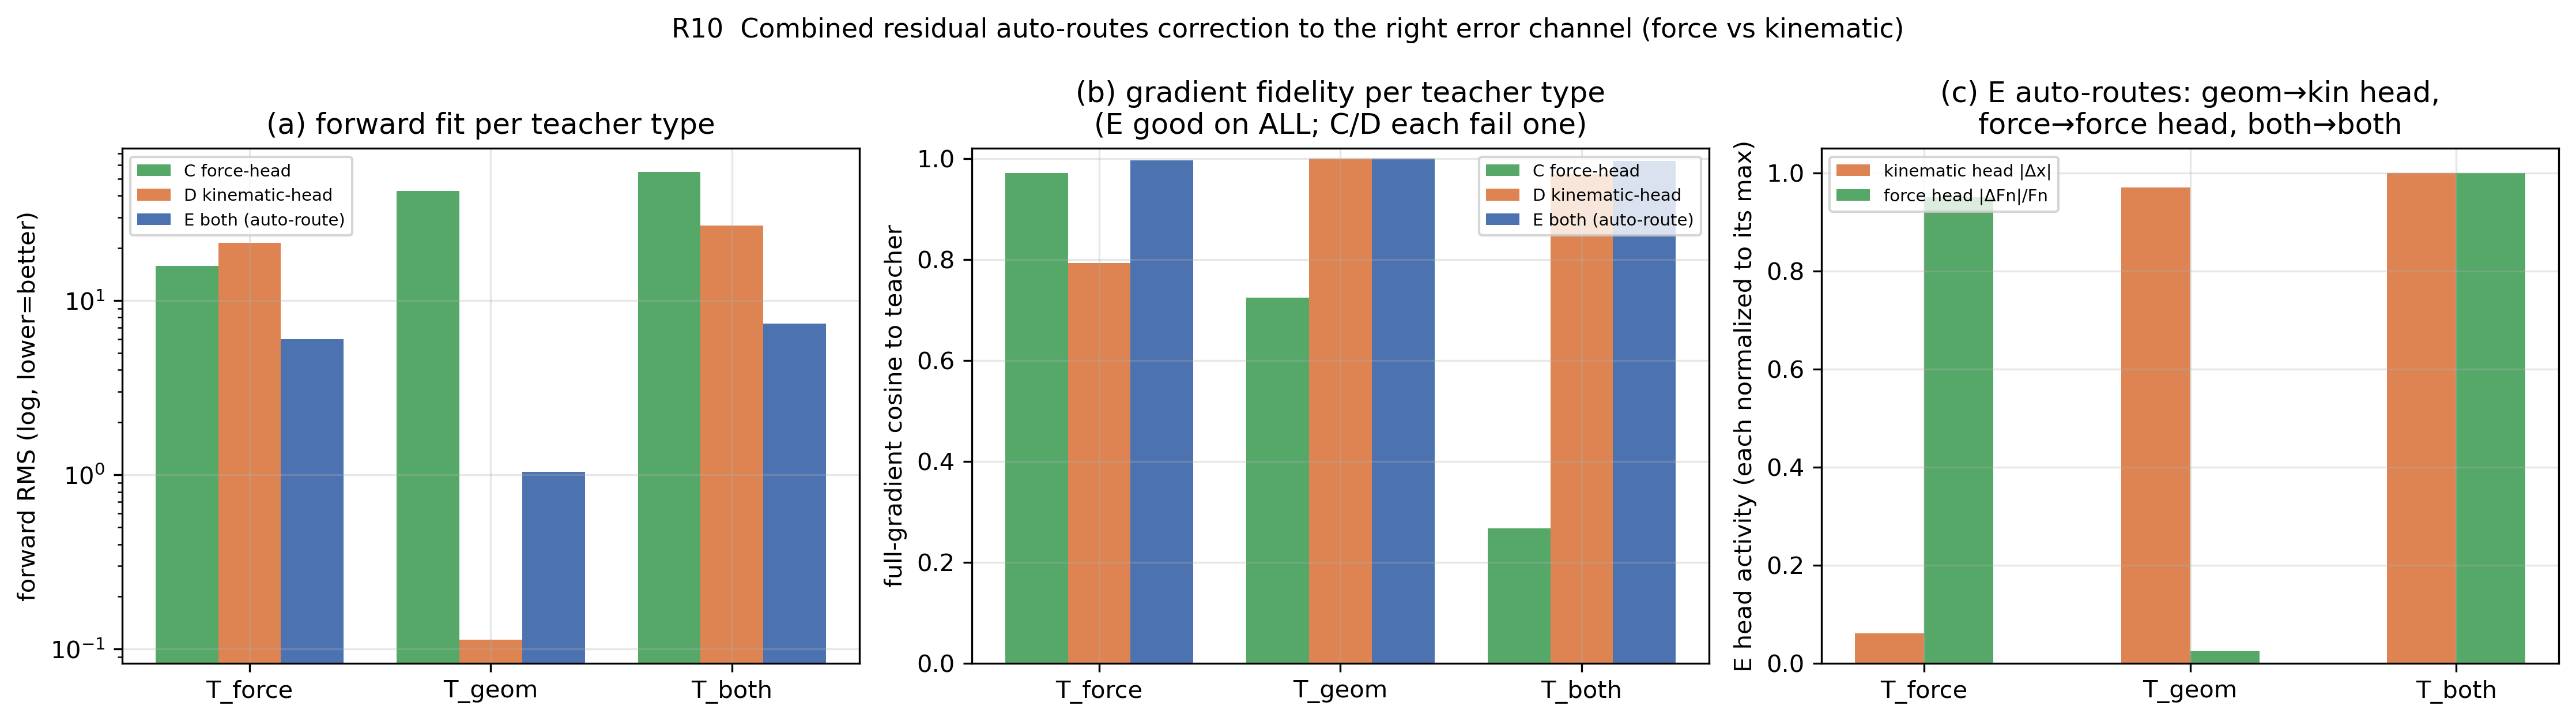
\includegraphics[width=0.97\textwidth]{R10_combined_residual.png}
  \caption{力 $+$ 运动学双头组合残差自动路由。左/中：单头各栽一种失配，双头在三类 teacher 上前向与梯度均最优。右：双头头活跃度随 teacher 自动切换——几何$\to$运动学头、参数$\to$力头、两者$\to$并用。}
  \label{fig:r10}
\end{figure}

\begin{figure}[htbp]
  \centering
  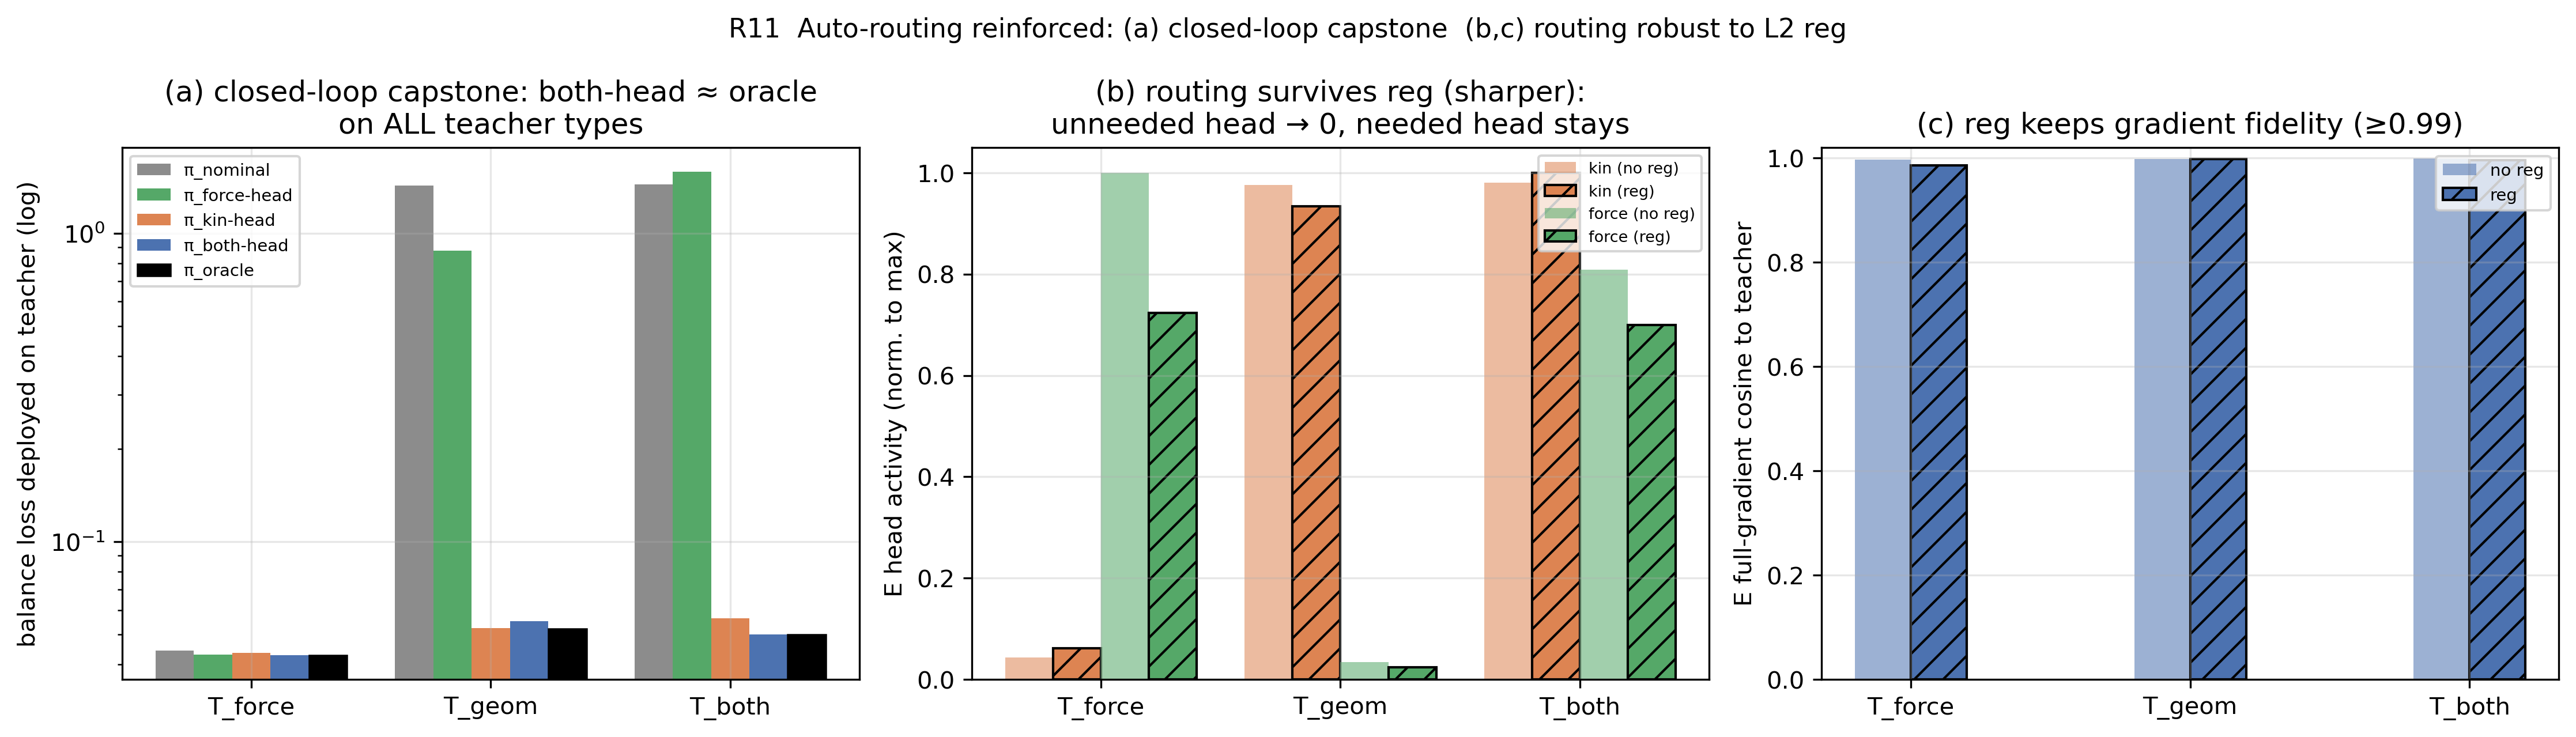
\includegraphics[width=0.97\textwidth]{R11_routing_capstone.png}
  \caption{双头路由加固。左：闭环 capstone——双头策略部署三种 teacher 全 $\approx$ oracle，几何盲的 nominal/力头在几何失配上崩。中/右：加 $L_2$ 正则后路由仍稳且更锐，梯度保真 $\ge$0.99，证明自动路由非偶然。}
  \label{fig:r11}
\end{figure}

\FloatBarrier
\subsection{残差选型总表}

\cref{tab:summary} 汇总全文主线：\textbf{残差的参数化位置必须与失配的物理类型匹配}。

\begin{table}[htbp]
  \centering
  \caption{按失配类型的残差选型总表（最优形式 / 错配失败模式 / 梯度与闭环结果）}
  \label{tab:summary}
  \small\setlength{\tabcolsep}{4pt}
  \renewcommand{\arraystretch}{1.15}
  \begin{tabular}{p{2.4cm}p{2.5cm}p{3.4cm}p{3.0cm}p{3.0cm}}
    \toprule
    失配类型 & 最优残差 & 错配失败模式 & 梯度结果 & 闭环结果 \\
    \midrule
    参数/力律 & 接触力残差 & 加速度残差前向准却梯度差；自由残差闭环最差 & 接触力残差余弦 0.998 $>$ 加速度 0.969 & 约束残差 $\approx$oracle；自由残差最差 \\
    小几何（力臂未翻转）& 接触力残差 & 自由残差把姿态梯度腐蚀到比 nominal 还差 & 接触力残差姿态余弦 0.978 vs 自由 0.927 & ---（仅梯度层面）\\
    极端几何（力臂翻转）& 运动学残差 & 接触力残差结构失明、从最优变最差 & 运动学残差余弦 1.00；接触力残差 0.28 & 运动学残差 $\approx$oracle；力残差/nominal 崩 \\
    未知/混合 & 双头组合 & 单头各栽一种（力头几何盲、姿态变号）& 双头三类 teacher 全 $\ge$0.995 & 双头三类 teacher 全 $\approx$oracle \\
    \bottomrule
  \end{tabular}
\end{table}

% ===================== 五、结论 =====================
\FloatBarrier
\section{结论}

本文面向可微物理从无人机到四足的迁移，聚焦"物理模型$+$神经残差"路线的\textbf{梯度保真}问题，在最小可微 SRBM 上系统比较了五种残差形式。借助"参数失配可微 teacher、真梯度可解析"的设计，本文给出可直接量化的梯度保真证据，得到一条贯穿始终的原理：\textbf{残差必须参数化在误差真正发生的物理位置}——力律误差用接触力残差、几何误差用运动学残差；放对地方则前向与梯度俱佳、可迁移，放错地方则前向能凑、梯度必崩，且该失败在闭环策略质量上被放大。沿此原理，本文（1）定量复现"前向 $\neq$ 梯度"并给出反例；（2）以接触门控、平滑摩擦锥、乘性限幅近乎零（梯度）成本地保证物理合法；（3）以力臂符号翻转\textbf{界定}物理结构的适用边界；（4）以双头自动路由在未知失配下统一三类失配，并以闭环 capstone 与正则化鲁棒性确证。

本文局限亦需明确。其一，全部实验在\textbf{最小 SRBM} 与\textbf{监督设定}下完成；"真梯度可解析"是使梯度保真\emph{可度量}的方法学便利，而真实 sim-to-real 中真梯度不可得，需\textbf{状态对齐}（用非可微高保真仿真器校正、其等价于无人机 GDecay 的推广）方能落地，引入该不可微环节后结论尚不可预判。其二，闭环验证采用的平衡任务对参数误差\textbf{反馈鲁棒}、且在几何翻转点支撑基退化而奇异，故闭环只作定性佐证、确定性结论以梯度量为准；更具区分度的前馈/失稳边界任务（精确轨迹、大扰动恢复、动态机动）有待设计。其三，尚缺真正抬腿的 stepping 步态与真机验证。未来工作将沿状态对齐、逐头自适应正则、以及向真实四足平台的迁移展开。尽管如此，本文给出的"残差选型$=$误差通道匹配"原理与可复现的最小实验，对可微物理在一切含接触系统上的迁移具有一般性的参考价值。

% ===================== 参考文献 =====================
\renewcommand{\refname}{参考文献：}
\begin{thebibliography}{99}
\small
\bibitem{ref8} Kaufmann E, Bauersfeld L, Loquercio A, et al. Champion-level Drone Racing Using Deep Reinforcement Learning[J]. Nature, 2023, 620(7976): 982-987.
\bibitem{ref11} Song Y, Romero A, Muller M, et al. Reaching the Limit in Autonomous Racing: Optimal Control versus Reinforcement Learning[J]. Science Robotics, 2023, 8(82): eadg1462.
\bibitem{ref13} Song Y, Kim S, Scaramuzza D. Learning Quadruped Locomotion Using Differentiable Simulation[C]//Conference on Robot Learning (CoRL). 2024.
\bibitem{ref14} Zhang Y, Hu Y, Song Y, et al. Back to Newton's Laws: Learning Vision-based Agile Flight via Differentiable Physics[J]. Nature Machine Intelligence, 2025, 7: 462-472.
\bibitem{ref12} Metz L, Freeman C D, Schoenholz S S, et al. Gradients are Not All You Need[J]. arXiv preprint arXiv:2111.05803, 2022.
\bibitem{ref29} Hu Y, Anderson L, Li T M, et al. DiffTaichi: Differentiable Programming for Physical Simulation[C]//International Conference on Learning Representations (ICLR). 2020.
\bibitem{refshac} Xu J, Makoviychuk V, Narang Y, et al. Accelerated Policy Learning with Parallel Differentiable Simulation[C]//International Conference on Learning Representations (ICLR). 2022.
\bibitem{refgeilinger} Geilinger M, Hahn D, Zehnder J, et al. ADD: Analytically Differentiable Dynamics for Multi-body Systems with Frictional Contact[J]. ACM Transactions on Graphics, 2020, 39(6): 1-15.
\bibitem{refsuh} Suh H J T, Simchowitz M, Zhang K, et al. Do Differentiable Simulators Give Better Policy Gradients?[C]//International Conference on Machine Learning (ICML). 2022.
\bibitem{refdiffsim2real} Bagajo J, Schwarke C, et al. Deploying Quadrupedal Locomotion Policies Purely Trained in Differentiable Simulation[C]//CoRL Workshop. 2024. arXiv:2411.02189.
\bibitem{refresidual} Ajay A, Wu J, Fazeli N, et al. Augmenting Physical Simulators with Stochastic Neural Networks[C]//IEEE/RSJ IROS. 2018.
\bibitem{refsource} Zhang Y, Hu Y, Song Y, et al. Back to Newton's Laws: Learning Vision-based Agile Flight via Differentiable Physics[J]. arXiv preprint arXiv:2407.10648, 2024.
\end{thebibliography}

\end{document}
